\documentclass[11pt]{article}

%--------------------------------------------------
% PACKAGES
%--------------------------------------------------
\usepackage[margin=1in]{geometry}  % Adjust page margins
\usepackage{amsmath,amssymb}       % Math packages
\usepackage{graphicx}              % For including graphics
\usepackage{hyperref}              % For clickable hyperlinks in document
\usepackage[numbers]{natbib}                % For better referencing/citations
% \usepackage{...}                 % Add any extra packages you need
\bibliographystyle{plainnat} % or another style if you prefer

%--------------------------------------------------
% TITLE
%--------------------------------------------------
\title{Removing Noise from Chaotic Dynamical Systems To Improve Accuracy of Takens Embedding and HAVOK}
\author{Igor Świerlikowski \\
	Maastricht University \\
	\texttt{i.swierlikowski@student.maastrichtuniversity.nl}}
\date{\today}

\begin{document}
	
	\maketitle
	
	%--------------------------------------------------
	% ABSTRACT
	%--------------------------------------------------
	\begin{abstract}
		This report explores the process of denoising chaotic dynamical systems and demonstrates the use of Takens Embedding and the HAVOK method for reconstructing and analyzing the underlying dynamics. I propose a framework for removing noise from chaotic signals and test the approach on the Lorenz Attractor system. My experiments show how these methods can improve the characterization of chaotic attractors and enhance predictability in data-driven models.
	\end{abstract}
	
	%--------------------------------------------------
	% KEYWORDS (optional)
	%--------------------------------------------------
	%\begin{keywords}
	%  chaos, dynamical systems, Takens embedding, HAVOK, noise removal
	%\end{keywords}
	
	%--------------------------------------------------
	% TABLE OF CONTENTS (optional)
	%--------------------------------------------------
	%\tableofcontents
	%\newpage
	
	%--------------------------------------------------
	% 1. INTRODUCTION
	%--------------------------------------------------
	\section{Introduction}
	Chaotic dynamical systems are prevalent in many fields, including physics, biology, and engineering. Despite their deterministic nature, chaos arises due to sensitive dependence on initial conditions, leading to behavior that appears random and is difficult to predict over long time horizons. One approach to characterizing such complexity is the Hankel Alternative View of Koopman (HAVOK) method \citep{brunton2017}, which seeks to decompose complex nonlinear systems into a mostly linear framework with identifiable nonlinear forcing terms. This decomposition can then be leveraged for better forecasting and analysis.
	
	In practice, measurement noise is often unavoidable when studying chaotic systems. Such noise can obscure the underlying chaotic behavior and complicate procedures like Takens Embedding, which is known to be highly sensitive to even small fluctuations. Consequently, efficient denoising techniques are critical for accurately reconstructing and predicting the true dynamics of these systems.
	
	In this report, we focus on one main technique for analyzing chaotic systems:
	\begin{itemize}
		\item \textbf{HAVOK Method}: A data-driven approach for decomposing time series into dominant modes and dynamical features. HAVOK begins with a time-delay Hankel matrix (as part of Takens Embedding) and applies Singular Value Decomposition (SVD). Afterwards, it uses Sparse Identification of Nonlinear Dynamics (SINDY) \citep{brunton2015} to represent the system with a predominantly linear component and a separate nonlinear forcing term.
	\end{itemize}
	
	When this method is combined with a suitable denoising strategy, we can recover essential features of the underlying chaotic dynamics and potentially forecast intermittent events, such as lobe switching in the Lorenz system.
	
	%--------------------------------------------------
	% 2. METHODOLOGY AND EXPERIMENTS
	%--------------------------------------------------
	\section{Methodology and Experiments}
	
	\subsection{Data Description}
	In these experiments, I work exclusively with the Lorenz system, given by the following set of ordinary differential equations:
	\begin{equation}
		\begin{aligned}
			\frac{dx}{dt} &= \sigma (y - x),\\
			\frac{dy}{dt} &= x(\rho - z) - y,\\
			\frac{dz}{dt} &= xy - \beta z,
		\end{aligned}
		\label{eq:lorenz}
	\end{equation}
	where the classical parameter set is
	\[
	\sigma = 10, \quad \rho = 28, \quad \beta = \frac{8}{3}.
	\]
	For the experiments, the Lorenz system is evolved from \(t_0 = 0\) to \(t_1 = 50\) with a time step \(\Delta t = 0.001\). The initial conditions are set to \((x, y, z) = (-8, 8, 27)\). Numerical integration is carried out in MATLAB using the \texttt{ode45} solver with a strict error tolerance of \(10^{-12}\).
	
	To simulate measurement noise, Gaussian or uniform noise is added to the time series \emph{after} the system evolution is completed, thus modeling realistic sensor or measurement errors rather than influencing the underlying dynamics directly.
	
	\subsection{Noise Removal Techniques}
	Three primary methods are evaluated for noise removal:
	\begin{itemize}
		\item \textbf{Moving Average} - a simple method with only one parameter \(window size\), which simply takes the average of its surrounding measurements in hopes of smoothing out the vector.
		\item \textbf{Savitzky--Golay} - instead of taking the average of surrounding data points like Moving Average, this method fits a low-degree polynomial to a set of neighboring points. It does so by finding coefficients that minimize the squared error between the polynomial and actual data in window. Its parameters are \(window size\) and \(order\) to specify the polynomial's order.
		\item \textbf{Wavelet Denoising}\citep{luo2012} - the most interesting method so far. It follows a method similar to Fourier Denoising, but instead performing a Discrete Fourier Transform where we would try fitting sin and cosine waves to our signal, we apply the Discrete Wavelet Transform and fit wavelets instead. This returns us a table of wavelets and their corresponding frequencies. To denoise, we simply cutoff these wavelets once we reach a high enough frequency - since that's where noise tends to reside. So far I have been using a \(wdenoise()\) method from the \(Wavelet Toolbox\) in MATLAB,which has no parameters but I'm planning to implement my own method in the upcoming semester.
	\end{itemize}
	These methods were selected to cover a range of filtering techniques and to evaluate their relative performance in preserving the chaotic structure while reducing noise. Furthermore all of these method's parameters were optimized across 15 different noise samples to ensure minimal errors in an unknown environment as well as a fair comparison. 
	
	\subsection{Takens Embedding}
	Takens Embedding creates a delay-embedded attractor from time series data. In the HAVOK framework, this procedure is realized by constructing a Hankel matrix of time-delayed coordinates. I closely follow the parameter choices outlined in \citep{brunton2017}:
	\begin{itemize}
		\item An embedding dimension (number of rows in the Hankel matrix) of 100.
		\item A delay time of 0.001, matching the numerical integration time step.
	\end{itemize}
	Future experiments will explore how changing these parameters can improve robustness against noise.
	
	\subsection{HAVOK Method}
	Once the Hankel matrix is formed, the next step is to perform SVD, yielding matrices \(U\), \(\Sigma\), and \(V^T\). Let \(\mathbf{v}(t)\) denote the relevant row components of \(V\). In the HAVOK procedure:
	\begin{itemize}
		\item We select the first \(r\) rows of \(V\) (i.e., the most dominant modes). Following the recommendation in \citep{brunton2017}, \(r\) is typically chosen as 15 in this work.
		\item A sparse regression (SINDY) is applied to the first \(r-1\) rows, while the \(r\)-th row is treated as an intermittent forcing term.
	\end{itemize}
	Hence, we arrive at a nearly linear system of the form:
	\begin{equation}
		\frac{d}{dt}\mathbf{v}(t) = A\,\mathbf{v}(t) + B\,v_r(t),
		\label{eq:havok}
	\end{equation}
	where \(A\) and \(B\) are matrices identified through sparse regression, and \(v_r(t)\) is the last mode representing nonlinear forcing.
	
	\subsection{Error Measure}
	To evaluate how our reconstructions perform in comparison to the original/noisy data, we need to find a way to compare our systems and create a fitting error measure. It must be able to compare the V matrix of both reconstructions. To do so I used the error measure of:
	
	\begin{equation}
		\text{error}_x = \sqrt{\sum \left( V_x(t_{\text{span}},1:r) - v_{\text{sim}}(t_{\text{span}},1:r) \right)^2 }
	\end{equation}
	 
	
	\subsection{Experimental Procedure}
	In summary, the experiments follow this pipeline:
	\begin{enumerate}
		\item \textbf{Data Generation}: Numerically integrate the Lorenz system over \([0,50]\) using \(\Delta t = 0.001\).
		\item \textbf{Noise Addition}: Inject Gaussian or uniform noise after integration.
		\item \textbf{Denoising}: Apply one of the chosen noise removal techniques (Moving Average, Savitzky--Golay, or Wavelet).
		\item \textbf{Takens Embedding \& HAVOK}: Construct the Hankel matrix, perform SVD, apply SINDY to form the HAVOK model.
		\item \textbf{Analysis}: Compare the reconstructed attractors, measure predictive performance, and assess sensitivity to noise.
	\end{enumerate}
	
	%--------------------------------------------------
	% 3. RESULTS
	%--------------------------------------------------
	\section{Results}
	
	\subsection{Investigating the cause of poor performance}
	My first experiment included me adding a tiny bit of noise to the system(sd = 0.01) to see if the delay embedding is the issue, or if its only finds trouble when it tries linearizing it. As we can see in the figure attached, the delay embedded attractor looked almost the same and it only started showing effects of the noise sensitivity once we tried reconstructing it with the HAVOK method.
	
	\begin{figure}
		\centering
		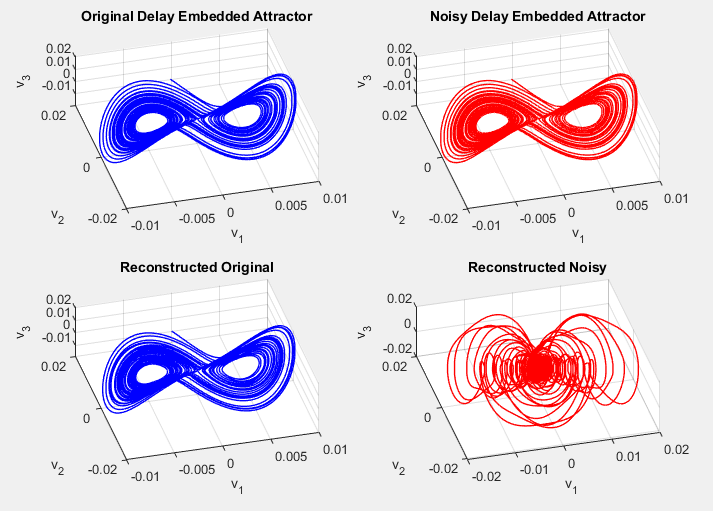
\includegraphics[width=0.7\linewidth]{Figure3}
		\caption{Comparing the original/noisy delay embedded attractors and their reconstruction}
		\label{fig:figure1}
	\end{figure}
	
	
	
	\subsection{Noise Removal Performance}
	This experiment was simply applying Gaussian noise with sd of 0.01 (very low) and mean of 0 to the results of the numerical integration of the Lorenz system and then smoothing it out using all of the previously described methods to see how well each of them performed. Then I calculated the RMSE of each sample as well as visually inspected them to see which one managed to get the closest to the original wave.
	
	\begin{figure}
		\centering
		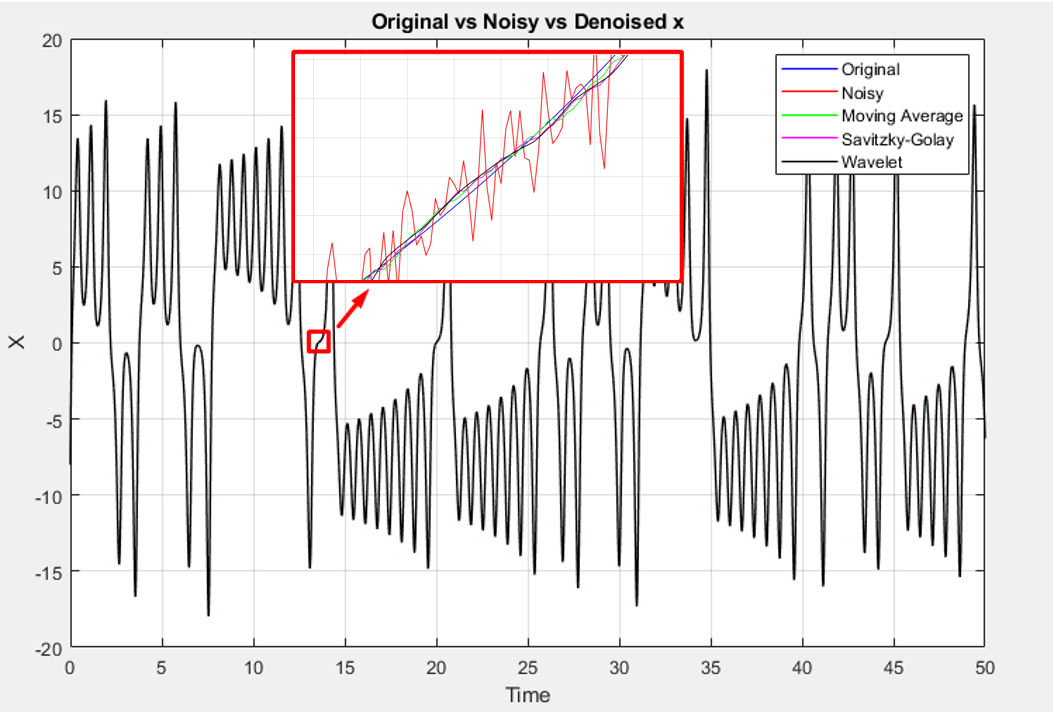
\includegraphics[width=0.7\linewidth]{Figure1}
		\caption{Graph of X to Time of the lorenz wave, when adding noise and after denoising, with a zoom in}
		\label{fig:figure2}
	\end{figure}
	
	\begin{figure}
		\centering
		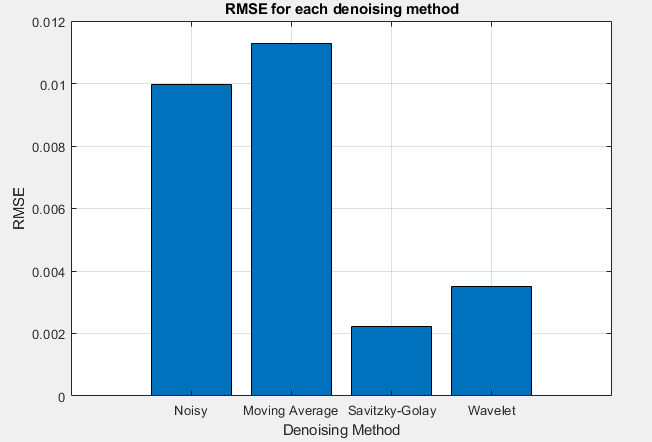
\includegraphics[width=0.7\linewidth]{Figure2}
		\caption{Bar chart of RMSE to denoising method to visualize the average Root Mean Square Error for the methods}
		\label{fig:figure3}
	\end{figure}
	
	
	

	
	\subsection{Denoised Havok Reconstructions}
	Having tested which noise reduction method performed the best in getting as close to the time-series as possible, we will now test out if they will also perform similarly with the HAVOK reconstruction or if there is more to it than just getting as close to the line as possible. The data used is the same as in 3.2. The error metric used in figure 5 was explained in section 2.5
	
	\begin{figure}
		\centering
		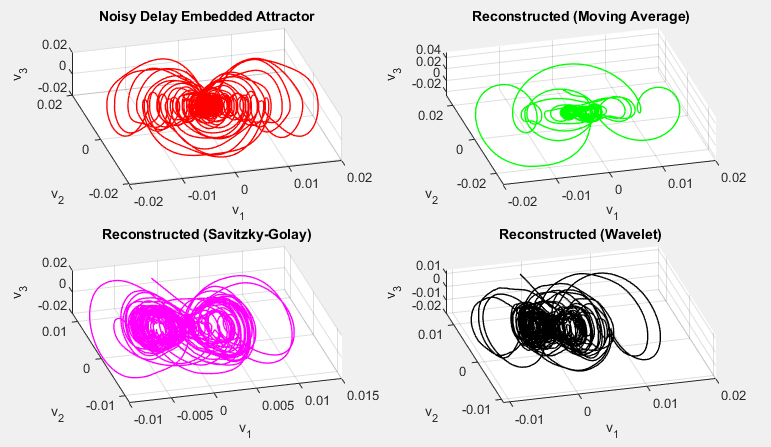
\includegraphics[width=0.7\linewidth]{Figure4}
		\caption{The noisy delay embedded attractor compared to it's denoised verision}
		\label{fig:figure4}
	\end{figure}
	
	\begin{figure}
		\centering
		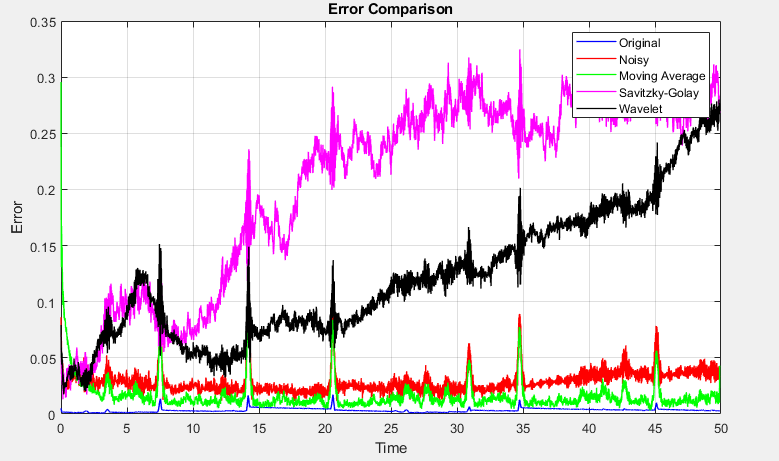
\includegraphics[width=0.7\linewidth]{Figure5}
		\caption{The error (from section 3.5) of each denoising method plotted against the time}
		\label{fig:figure5}
	\end{figure}
	
	
	%--------------------------------------------------
	% 4. DISCUSSION
	%--------------------------------------------------
	\section{Discussion}
	
	\subsection{Investigating the cause of poor performance}
	Given the results visible in Figure1, we can say with confidence that the problem doesn't lie within Takens Embedding but instead , once we try to linearize the system. This makes sense since linear systems do struggle with fitting higher frequency oscillations, and the only reason lobe switching is possible in the Lorenz system is due to the non-linear component. Given these results I think that a possible way of reducing the noise sensitivity would be to increase \(r\), aka the parameter in HAVOK which tell us how many equations show describe the system, but that's research that Im planning to continue in the next semester.
	
	\subsection{Noise Removal Performance}
	As we can see in Figure3, Savitzky-Golay and Wavelet Denoising seem to have way less error than the noisy system by itself. Moving Average however, has even more error than just the noisy data. Because of this I will refrain from researching deeper into moving average and instead focus on Savitzky-Golay, and primarly, Wavelet Denoising as my main methods for the next semester. 
	
	\subsection{Denoised Havok Reconstructions}
	Figure4 shows clear improvement in resemblance to the original delay embedded attractor using the Savitzky-Golay and Wavelet reconstruction methods. In both of them one can find the two cleary separated lobes although a lot of noise influence is still visible. I will continue working with these methods to further enhance them in the next semester, but will put most of my focus in Wavelet Denoising since it has a lot more room for improvement, like using different wavelets instead of the default one.
	
	\subsection{Error Measure}
	As we can see from our results in Figure5, our error measure is very poor. According to it, Savitzky Golay and Wavelet Denoising should be the two worst methods on our list and instead they outperformed the rest by far. This is due to the fact, that our error measure treats every row in the V matrix equally while HAVOK - doesn't. When taking a colser look at the rows of V (see figure 6), we can see that the rows of the first matrix match quite closely to our desired wave, but the further we go, the more visible noise is - but also the less important it is for our reconstruction. This suggest that we need to improve our error measure so we can more accurately compare our systems.
	
	\begin{figure}
		\centering
		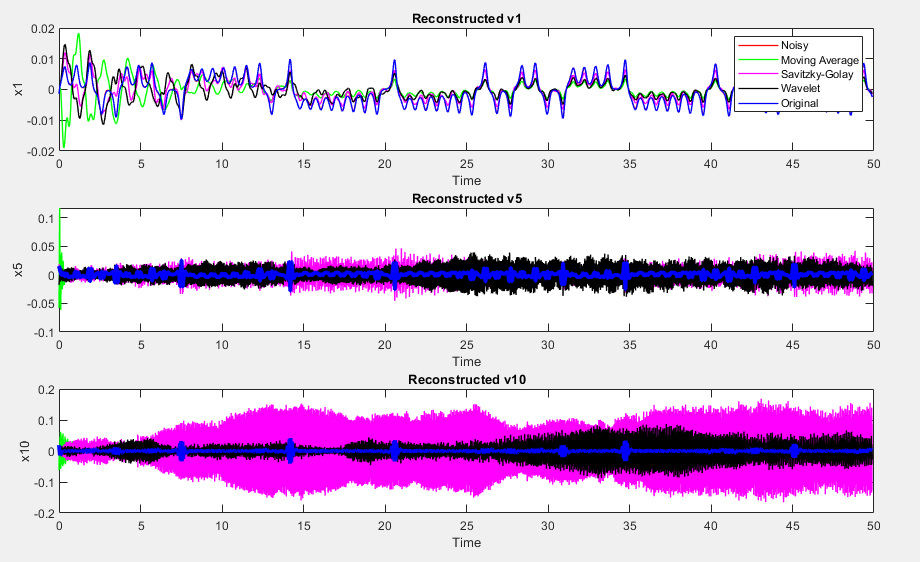
\includegraphics[width=0.7\linewidth]{Figure6}
		\caption{The first, fifth and 10th rows of V's from the reconstructions, plotted against time}
		\label{fig:figure6}
	\end{figure}
	
	
	%--------------------------------------------------
	% 5. RESEARCH QUESTIONS
	%--------------------------------------------------
	\section{Research Questions}
	To guide this study next semester, I pose the following research questions:
	\begin{enumerate}
		\item How can we effectively remove measurement noise from a chaotic time series while preserving the underlying structure?
		\item To what extent does noise removal improve the accuracy of the HAVOK method for reconstructing the attractor?
		\item How does the HAVOK method, combined with noise-reduced data, improve our ability to predict and model chaotic systems?
		\item What are the limitations of the proposed denoising techniques when applied to different types and levels of noise?
		\item What different error measure can we use to better visualize our results?
	\end{enumerate}
	
	%--------------------------------------------------
	% 6. CONCLUSION
	%--------------------------------------------------
	\section{Conclusion}
	In this study, I explored methods for removing noise from chaotic dynamical systems, specifically in the context of the Lorenz attractor, to improve the accuracy of the Takens Embedding and HAVOK reconstruction. Through the application of three noise reduction techniques—Moving Average, Savitzky-Golay, and Wavelet Denoising—I evaluated their performance in preserving the underlying chaotic structure while minimizing the impact of noise.
	
	The results demonstrated that Moving Average was ineffective in reducing noise while preserving the chaotic features, whereas both Savitzky-Golay and Wavelet Denoising performed significantly better. The HAVOK reconstructions based on these methods retained the overall attractor shape, although some sensitivity to noise remained. Additionally, an investigation into the cause of poor HAVOK performance revealed that the challenge lies not in Takens Embedding itself but in the process of linearizing the system. This suggests potential future improvements, such as increasing the HAVOK model order \(r\), to better capture nonlinear dynamics.
	
	Furthermore, the analysis highlighted a flaw in the error measure used to compare different noise reduction techniques. Since HAVOK prioritizes certain modes over others, a simple sum-of-squared-errors approach across all components of \(V\) does not accurately reflect reconstruction quality. A more refined error metric that accounts for HAVOK’s mode importance will be explored in future research.
	
	Moving forward, my next semester's work will focus on refining the denoising techniques—particularly Wavelet Denoising—by experimenting with different wavelet functions and thresholding strategies. Additionally, I will investigate alternative error metrics to more accurately assess reconstruction quality. Finally, I will analyze whether noise reduction significantly enhances HAVOK’s predictive capabilities for chaotic time series.
	
	By improving noise removal strategies and refining the HAVOK framework, this research contributes to the broader goal of making chaotic systems more accessible for data-driven modeling and prediction, which has applications in fields ranging from meteorology to finance and biological systems.
	
	%--------------------------------------------------
	% REFERENCES
	%--------------------------------------------------

	\begin{thebibliography}{99}
		
		\bibitem{brunton2017}
		Brunton, S. L., Brunton, B. W., Proctor, J. L., \& Kutz, J. N. (2017). \textit{Chaos as an intermittently forced linear system}. Nature Communications.
		
		\bibitem{brunton2015}
		Brunton, S. L., Proctor, J.L., \& Kutz, J. N. (2017). \textit{Discovering governing equations from data: Sparse identification of nonlinear dynamical systems}. PNAS.
		
		\bibitem{luo2012}
		Luo, G., \& Zhang, D. (2012). \textit{Wavelet Denoising}. In \textit{Advances in Wavelet Theory and Their Applications in Engineering, Physics and Technology}. IntechOpen. https://doi.org/10.5772/37424
		
		% Add more references as needed
		
	\end{thebibliography}
	
\end{document}
